\section{Release notes}

\subsection{Changes to the previous version}
This is where changes should be listed.



\subsection{Corrections}
A mistake was discovered in NVU1.0 for the equation used to describe the \gls{K} concentration in the synaptic cleft. The original equation subtracted the change in astrocytic \gls{K} concentration from the \gls{K} influx from the neuron. This was incorrect since not all channels lead from the astrocyte to the synaptic cleft. The BK-channel describes the flux from the astrocyte to the perivascular space, and therefore this flux was added to the equation. Fortunately, this mistake led to very small changes, and it did not significantly change the model outcomes. Figure \ref{fig:cordif} shows the old and the corrected results for the flux through the BK-channel, and it is clear that they practically overlap. 

\begin{figure}[h!]
	\centering
	\tiny  
	\setlength\figureheight{5 cm} 
	\setlength\figurewidth{15 cm}
	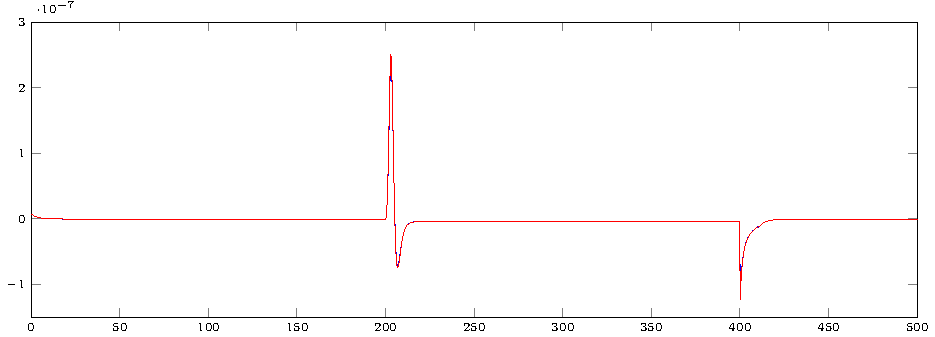
\includegraphics[width=15cm]{figures/diff_cor.pdf}
	\caption{The flux through the BK-channel in \textmu M m/s for the old (blue) and corrected (red) simulation }
	\label{fig:cordif}
\end{figure}
